\documentclass[10pt]{article}
\pagestyle{empty}
\usepackage{hyperref}
\usepackage{harvard}
\usepackage{amsthm,amsfonts,amsmath}
\usepackage{enumitem}
%\usepackage[pdftex]{graphicx}%%for Pdftex
\usepackage{graphicx}%%for Latex
\usepackage{multirow}
\usepackage{bbm}
\usepackage{amssymb}
\usepackage{amsthm}
\usepackage{url}
\usepackage{mathrsfs}
\usepackage{appendix}
%\usepackage[pdftex]{graphicx}
%\usepackage{subfigure}
%\usepackage{multicol}
%\usepackage{color}
\usepackage{algorithm}
\usepackage{algorithmic}
\usepackage{setspace}

%set dimensions of columns, gap between columns, and paragraph indent 
\setlength{\textheight}{8.5in}
\setlength{\textwidth}{5in}
\setlength{\headheight}{0cm}
\setlength{\headsep}{0cm}
%\setlength{\footheight}{0.0in}
\setlength{\parindent}{1pc}

%macro
%%%%%%%%%%%%%%%%%%%%%%%%%%%%%%%%%%%%%%%%%%%%%%%%%%%%%%%%%%%%%%%%%%%%%%%%%
\hyphenation{con-tin-u-ous-time con-tin-u-ous bank-rupt-cy}
\hyphenation{Lebes-gue} \hyphenation{ter-mi-nol-o-gy}
%%%%%%%%%%%%%%%%%%%%%%%%%%%%%%%%%%%%%%%%%%%%%%%%%%%%%%%%%%%%%%%%%%%%%%%%%
\newcommand{\bbr}{\mathbb{R}}  %black board bold \mathbb{R}
\newcommand{\bbn}{\mathbb{N}}
\newcommand{\bbp}{\mathbb{P}}
\newcommand{\bY}{\mathbf{Y}}
\newcommand{\mun}{\lceil \mu n \rceil}
\newcommand{\etan}{\lceil \eta n \rceil}
\newcommand{\bbq}{\mathbb{Q}}
\newcommand{\wQ}{\widetilde{\bbp}}%change per Prof. Lai's request to alleviate confusion
\newcommand{\wq}{\widetilde{p}}%change per Prof. Lai's request to alleviate confusion
\newcommand{\wY}{\widetilde{Y}}
\newcommand{\wX}{\widetilde{X}}
\newcommand{\ow}{\overline{w}}
\newcommand{\wht}{\widehat}
\newcommand{\var}{\ensuremath{\mathbb Var}}
\newcommand{\wbY}{\widetilde{\bY}}
\newcommand{\abs}[1]{\lvert#1\rvert}
\newcommand{\D}{\mathbb{D}}
\newcommand{\G}{\mathbb{G}}
\newcommand{\bbe}{\mathbb{E}}
\newcommand{\F}{\mathbb{F}}
\newcommand{\HH}{\mathbb{H}}
\newcommand{\bbj}{\mathbb{J}}
\newcommand{\bbz}{\mathbb{Z}}
\newcommand{\bbs}{\mathbb{S}}
\newcommand{\C}{\mathbb{C}}
\newcommand{\bu}{\mathbf{u}}
\newcommand{\bx}{\mathbf{x}}
\newcommand{\fn}{\footnote}
\newcommand{\ci}{\citeasnoun}
\newcommand{\om}{\omega}
\newcommand{\la}{\lambda}
\newcommand{\tla}{\tilde{\lambda}}
\newcommand{\doth}{f}
\renewcommand{\labelenumi}{\roman{enumi}}
\newcommand{\ps}{P}
\newcommand{\pss}{\ensuremath{\mathbf{p}}} %small boldface
\newcommand{\pmq}{\ensuremath{\mathbf{Q}}}
\newcommand{\pmqs}{\ensuremath{\mathbf{q}}}
\newcommand{\pas}{P-a.s. }
\newcommand{\pasm}{P\mbox{-a.s. }}
\newcommand{\asm}{\quad\mbox{a.s. }}
\newcommand{\cadlag}{c\`adl\`ag }
\newcommand{\fil}{\mathcal{F}}
\newcommand{\gcal}{\mathcal{G}}
\newcommand{\hcal}{\mathcal{H}}
\newcommand{\jcal}{\mathcal{J}}
\newcommand{\pcal}{\mathcal{P}}
\newcommand{\ecal}{\mathcal{E}}
\newcommand{\bcal}{\mathcal{B}}
\newcommand{\ical}{\mathcal{I}}
\newcommand{\scal}{\mathcal{S}}
\newcommand{\ncal}{\mathcal{N}}
\newcommand{\lcal}{\mathcal{L}}
\newcommand{\kcal}{\mathcal{K}}
\newcommand{\acal}{\mathcal{A}}
\newcommand{\mcal}{\mathcal{M}}
\newcommand{\rcal}{\mathcal{R}}
\newcommand{\tcal}{\mathcal{T}}
\newcommand{\ti}{\times}
\newcommand{\we}{\wedge}
\newcommand{\be}{\begin{equation}}
\newcommand{\ee}{\end{equation}}
\newcommand{\bew}{\begin{equation*}}
\newcommand{\eew}{\end{equation*}}
\newcommand{\uK}{\underline K}
\newcommand{\oK}{\overline K}
\renewcommand{\th}{\tilde{h}}
\newcommand{\imp}{\eta}
\newcommand{\xbar}{\overline{X}}
\newcommand{\Xij}{X_{i,j}}
\newcommand{\f}{\left}
\newcommand{\g}{\right}
\newcommand{\naiveest}{\wht{\sigma^2_n}}
\newcommand{\deltaest}{\wht{\sigma^2_d}}

%theorem style
\newtheorem{thm}{Theorem}
\newtheorem{cond}[thm]{Condition}
\newtheorem{defi}[thm]{Definition}
\newtheorem{algo}[thm]{Algorithm}
\newtheorem{prop}[thm]{Proposition}
\newtheorem{corollary}[thm]{Corollary}
\newtheorem{lem}[thm]{Lemma}
\newtheorem{rem}[thm]{Remark}
\newtheorem{ex}[thm]{Example}
\newtheorem{ass}[thm]{Assumption}

\begin{document}

%don't want date printed
\date{}

%make title bold and 14 pt font (Latex default is non-bold, 16pt) 
\title{\Large\bf Choice of the Randomization Unit in Online Controlled Experiment}

%for single author (just remove % characters)
%\author{Shaojie Deng \\
%  Microsoft \\
%  Redmond, WA, 98052}

%for two authors (this is what is printed)
%\author{
%\begin{tabular}[t]{c@{\extracolsep{8em}}c}
%Shaojie Deng  &  Roger Longbotham & Toby Walker & Ya Xu  \\
%  Microsoft & Microsoft & Microsoft & Microsoft 
%% alexdeng@microsoft.com & roger.longbotham@microsoft.com & toby.walker@microsoft.com & yaxu@microsoft.com 
%\end{tabular}
%}
\author{Shaojie Deng\footnote{Microsoft, Redmond, WA 98052, USA, email: {\tt alexdeng@microsoft.com}.}\;\;\;\; Roger Longbotham\footnote{Microsoft, Redmond, WA 98052, USA, email: {\tt roger.longbotham@microsoft.com}.}\;\;\;\; Toby Walker\footnote{Microsoft, Redmond, WA 98052, USA, email: {\tt toby.walker@microsoft.com}.}\;\;\;\; Ya Xu\footnote{Microsoft, Redmond, WA 98052, USA, email: {\tt yaxu@microsoft.com}.} } \normalsize

\date{September 8, 2010\\ This version: \today}
\maketitle

%So first page doesn't have a page number
\thispagestyle{empty}

\subsection*{Abstract}
Controlled experiment has been used widely to support data driven decision making for online businesses. By applying appropriate randomization of the experiment units, causal inference can be established. The choice of the experiment unit for randomization can vary. User and page view are two mostly used units. Moreover, the analysis unit is sometimes different from the experiment unit. There are pros and cons in choosing which experiment unit to use and the choice affects the downstream statistical analysis. In this paper, we compare the two experiment units and highlight the differences in related statistical analysis.     
\subsection*{Keywords}
Controlled experiment, Experimentation, A/B testing, randomization unit, Variance estimation. 


\section{Introduction}
[Todo]  Introduction section. 

The following paper is organized as follows. We firt introduce notation in Section \ref{notation}. In Section \ref{user}, we first review the two sample t-test for  metrics using user as the corresponding analysis unit. We then show delta method should be used when analysis unit is finer than user level and also gives a formula for the bias introduced should we fail to use delta method. In Section \ref{page}, we change gear to the case that the randomization unit is page view. In particular, we present the correct variance formula for the two layer randomization framework. In Section \ref{compare}, we discuss the pros and cons of different randomizaiton units. 
Section \ref{empirical} presents empirical results(or simulation results). Section \ref{conclusion} summarizes and concludes. 

\subsection{Notation}\label{notation}
Before going into the next section, we introduce notation and assumptions which will be consistently used through out this paper. Denote $n$ the total number of unique users. Let $X_{i,j}$ be the per-page measurement (e.g. number of clicks on ths page) on user $i$'s $j^{th}$ page view and $X_{i,j}$ has mean $\mu_i$ and variance $\sigma_i^2$.  Denote $K_i$ the total number of page views from user $i$ and $N = \sum_{i=1}^n K_i$ be the total number of page views. We assume for any $i$, $X_{i,j},j=1,\dots,K_i$ are i.i.d. and uniformly bounded above by some finite constant.  But we allow $(\mu_i,\sigma_i^2)$ to differ from user to user. We also assume $K_i,i=1,\dots,n$ are i.i.d. and independent of $(\mu_i,\sigma_i^2),i=1,\dots,n$. This last assmption may not be true in practice and need to be checked case by case. We have checked this assumption for some key metrics of web experiments using empirical data and this assumption is reasonable.


\section{User as Randomization Unit}\label{user}

\subsection{User Level Metrics}
This is the simple case. Brifely introduce the two sample t-test. Introduce necessary notations for following sections. 

\subsection{Page Level Metrics}
A page level metric can be denoted by:
\begin{align*}
\xbar= \frac{\sum_{i=1}^n\sum_{j=1}^{K_i} X_{i,j}}{N}.
\end{align*}
To estimate the varaince of $\xbar$, it is tempting to treat page level metrics $X_{i,j}$, $j=1,\dots,K_i$, $i=1,\dots,n$, as i.i.d. and $\xbar$ under this assumption is an average of i.i.d. samples so the variance of $\xbar$ can be easily estimated by
\begin{align*}
\frac{1}{N^2} \Bigl (\sum_{i=1}^n \sum_{j=1}^{K_i} (X_{i,j}-\overline{X})^2 \Bigr ).
\end{align*}
This estimator, which we call the \emph{naive} estimator,  is not consistent because unlike the fixed effect model, where the only randomness is from the noise of $X_{i,j}$. In our model the user effect $(\mu_i,\sigma_i^2)$ are also a random sample from a distribution. Nevertheless, it is true in our model that the user level measurement $(\sum_{i=1}^{K_i} X_{i,j}, K_i),i=1,\dots,n$ are i.i.d. By letting $Y_i = \sum_{i=1}^{K_i} X_{i,j}$ and express $\xbar$ as $\sum_{i=1}^n Y_i / \sum_{i=1}^n K_i$, it is then a straightforward application of the delta method to get an asymptotically consistent estimator for $\var \xbar$:
\begin{align*}
\frac{1}{n} \Bigl\{ \frac{1}{\wht{\bbe K_i}^2}\wht{\var Y_i} + \frac{\wht{\bbe Y_i}^2}{\wht{\bbe K_i}^4}\wht{\var K_i} - 2\frac{\wht{\bbe Y_i}}{\wht{\bbe K_i}^3} \wht{Cov(Y_i,K_i)} \Bigr\} 
\end{align*}
where these ``hatted'' quantities are the sample mean, variance or covariance. 

For asymptotic analysis, we will let $n\to \infty$ (so $N\to \infty$ a.s.). To normalize the naive estimator and delta method estimator, we multiply them by $n$ so that they will converge to some nonzero numbers.  We introduce the normalized naive estimator 
\begin{align}
\wht{\sigma^2_n} = n\frac{1}{N^2} \Bigl (\sum_{i=1}^n \sum_{j=1}^{K_i} (X_{i,j}-\overline{X})^2 \Bigr ).
\end{align}
and the normalized delta method estimator
\begin{align}
\wht{\sigma^2_d} = \frac{1}{\wht{\bbe K_i}^2}\wht{\var Y_i} + \frac{\wht{\bbe Y_i}^2}{\wht{\bbe K_i}^4}\wht{\var K_i} - 2\frac{\wht{\bbe Y_i}}{\wht{\bbe K_i}^3} \wht{Cov(Y_i,K_i)}
\end{align}
A natural question to ask is how biased is the naive estimator $\naiveest$ relative to the true normalized variance $n\var \xbar$. This is answered in the following theorem.
\begin{thm}\label{thm1.1}
Let $C = \frac{\bbe K_i^2}{(\bbe K_i)^2}$.  Then, as $n\to \infty$,
\begin{align}
n\var\xbar &\to C \var(\mu_i) + \bbe(\sigma^2_i)/\bbe (K_i)\label{truevar} \\
\deltaest & \to  C \var(\mu_i) + \bbe(\sigma^2_i)/\bbe (K_i)\label{deltalim}  \\
\naiveest & \to  \frac{1}{\bbe(K_i)} (\var(\mu_i)+\bbe(\sigma_i^2))\label{naivelim}.
\end{align}
Let $\rho:= \var(\mu_i)/(\var(\mu_i)+\bbe(\sigma^2_i))$ be the user effect coefficient(variances that explained by between user variation), then
\begin{align}
\frac{n\var (\xbar)}{\naiveest} \to  (\bbe(K_i)C - 1)\rho +1.
\end{align}
The convergence in \eqref{deltalim} and \eqref{naivelim} are  in probability. 
\end{thm}

\begin{proof}[Proof of Theorem \ref{thm1.1}.]
\eqref{deltalim} follows directly from the property of the delta method. To prove \eqref{truevar}, we first apply conditional variance formula by conditioning on $(\mu_i,\sigma_i^2, K_i, i=1,\dots,n)$. This gives
\begin{align*}
&\var \xbar =  \var  \Bigl( \bbe\Bigl(   \frac{\sum_{i=1}^n\sum_{j=1}^{K_i} X_{i,j}}{N} \Big| K_i,\mu_i,\sigma_i^2,  i=1,\dots,n\Bigr) \Bigr) \\
+&\bbe \Bigl(\var \Bigl( \frac{\sum_{i=1}^n\sum_{j=1}^{K_i} X_{i,j}}{N} \Big | K_i,\mu_i,\sigma_i^2,  i=1,\dots,n\Bigr)\Bigr) \notag\\
=&\var \Bigl(\frac{1}{N}\sum_{i=1}^n K_i \mu_i \Bigr)+\bbe \Bigl(\frac{1}{N^2}\sum_{i=1}^n K_i \sigma^2_i \Bigr).
\end{align*}
Let  $w_i = K_i/\sum_{i=1}^n K_i = K_i/N$. Since $K_i$ independent of $(\mu_i, \sigma^2_i)$ and $N/n \to \bbe {K_i}$ as $n\to \infty$, we can further simplify the right hand. First, by applying iterative expectation(frist conditioning on $w_1,\dots, w_n$), we have  
\begin{align}
n \bbe \Bigl(\frac{1}{N^2}\sum_{i=1}^n K_i \sigma^2_i \Bigr)  = \sum_{i=1}^n \bbe\Bigl( \frac{n}{N} w_i\sigma^2_i \Bigr) = \frac{1}{\bbe K_i}(\sum_{i=1}^n w_i)\bbe \sigma_i^2 = \frac{\bbe \sigma_i^2}{\bbe K_i} \label{withinterm}
\end{align}
where the second equality is by bounded convergence theorm(since $N/n \to \bbe {K_i}$ and $\sum w_i\sigma^2_i$ bounded) and the last equation is from $\sum w_i=1$. Since $(\mu_i, \sigma^2_i), {i=1,\dots, n}$ are i.i.d., 
\begin{align}
&n\var (\sum_{i=1}^n w_i \mu_i) = n\bbe (\var (\sum_{i=1}^n w_i \mu_i|w_1,\dots,w_n))+ n\var (\bbe (\sum_{i=1}^n w_i \mu_i|w_1,\dots,w_n)) \\
&=  n\bbe (\sum_{i=1}^n w_i^2 \var(\mu_i)) + n \var((\sum_{i=1}^n w_i)\bbe\mu_i ) = n\bbe(\sum_{i=1}^n w_i^2) \var (\mu_i) \label {betweenterm}
\end{align}
where the last equality is from the fact that the second term is $0$. By simple algebra, 
$n \sum_{i=1}^n w_i^2 =  \frac{\overline{K_i^2}}{\overline{K_i} \times \overline{K_i}}$, where $\overline{K_i^2}$ and $\overline{K_i}$ are sample mean of $K_i^2$ and $K_i$, respectively.
By strong law of large number, $\overline{K_i^2}\to \bbe K_i^2$ a.s., $\overline{K_i}\to \bbe K_i$ a.s., therefore $n \sum_{i=1}^n w_i^2 =  \frac{\bbe{K_i^2}}{(\bbe{K_i})^2}$ a.s. Combine this result with \eqref{withinterm} and \eqref{betweenterm}, we've proved \eqref{truevar}.

We now turn to the limit of $\naiveest$. 
\begin{align*}
 \naiveest &= n \frac{1}{N^2} \Bigl (\sum_{i=1}^n \sum_{j=1}^{K_i} (X_{i,j}-\overline{X})^2 \Bigr )= \frac{n}{N^2} \Bigl \{  \sum_{i=1}^n \sum_{j=1}^{K_i} X_{i,j}^2 - N \xbar^2 \Bigr\}\\
&\to   \lim_{n\to \infty} \Bigl(\frac{n^2}{N^2}\Bigr) \bbe \bigl(\sum_{j=1}^{K_i} \Xij^2 \bigr) -   \lim_{n\to \infty} \Bigl(\frac{n}{N}\Bigr) (\bbe \mu_i)^2 .
\end{align*}
The last limit is from $(1/n) \sum_{j=1}^{K_i} X_{i,j}^2 \to \bbe \bigl(\sum_{j=1}^{K_i} \Xij^2 \bigr)$ and $\xbar \to \bbe \mu_i$ a.s., both by the strong law of large number.
Using bounded convergence theroem and $N/n \to \bbe K_i$, and also $\bbe \bigl(\sum_{j=1}^{K_i} \Xij^2 \bigr)  = \bbe K_i \bbe X_{i,j}^2 = \bbe K_i (\bbe \mu_i^2 + \bbe \sigma_i^2)$,
\eqref{naivelim} follows.
\end{proof}




\section{Page View as Randomizaiton Unit}\label{page}
\subsection{A two layer randomization framework}
Now we consider the case that randomization is done by page view. Suppose ALL page views are randomly divided into different groups. By ALL page views we mean page views from all users that could show up. Under this framework, it is from the typical marginalization argument that we can treat page view level measurement as i.i.d. i.e., there is no user effect in the analysis because the page views are drawn from all users and no user selection variance is induced in this randomization scheme. Since page view level measurements are i.i.d., all statistical analysis no finer than page view level is therefore straightforward. 

The case that is of more interest is the following. We do not want to perform experiment on all users. Instead, we first randomly selected $n$ user from all the users in the universe. $n$ is usually only a small percentage of the total number $M$ of users in the universe so let us assume $M$ is infinity and hence the users are drawn independently. All the page views from these $n$ users are then randomly split into control and treatment. The goal is to make inference by comparing some metrics in control and treatment. 

We inherit all the notations from Part I. Suppose we are interested in page view level metrics $\xbar_r = \sum_{i=1}^n \sum_{j=1}^{{K_i}^{(r)}}X_{i,j}^{(r)}/N_r$ where $r=1,2$ stands for control and treatment. In Part I, we never consider the variance of both control and treatment together. This is because the control and treatment groups have different users and since randomization is based on user, the metrics of the two groups are therefore independent. As a result the variance of the metrics difference is simply the sum of the two variances of metric in each group.  What make things more complicated is that the current framework, control and treatment share the same group of $n$ users. It is the page view, not the user that is randomized into two groups. Due to this very fact, $\xbar_1$ and $\xbar_2$ are no longer independent. 


\subsection{Variance formula}
In this section we give the asymptotically unbiased estimator for $\var (\xbar_1-\xbar_2)$ when the page views are split into control and treatment with fixed weights. For simplicity, we first assume control and treatment have the same weights. But we will give the result for general case in the end of this Section. Under the same assumption as in Part I that number of page views $K_i$ are independent of $(\mu_i,\sigma_i^2)$. Then conditioned on $K_i$, $K_i^{r}$ follows from $binomial(K_i, 0.5)$ distribution. If we only consider one group, say control. Then the only difference between this framework and that of Section \ref{user} is that now $K_i^{r}$ follows from a different distribution(from $K_i$). But note that all the result in Section \ref{user} does not depend on the distribution of $K_i$. Therefore all results in Section \ref{user} directly apply on $\xbar_1$ (or $\xbar_2$). 

\begin{prop}\label{p_prop1}
Let $w_i^{(r)}=K_i^{(r)}/\sum_{i=1}^{n} K_i^{(r)} $. Assume $n\bbe (\sum_{i=1}^n {(w_i^{(r)})}^2)\to C$, $r=1,2$ as $n\to \infty$. Then for $r=1,2$
\begin{align}
\bbe(\naiveest_r) &\to  \frac{1}{\bbe(K_i^{(r)})} (\var(\mu_i)+\bbe(\sigma_i^2)) \label{p_naive}\\
\bbe (\deltaest_r) &\to C \var(\mu_i) + \bbe(\sigma^2_i)/\bbe (K_i^{(r)}) \label{p_delta}.
\end{align}
\end{prop}

What Proposition \ref{p_prop1} says is exactly that if we apply naive formula or delta method formula to one group, we will get asymptotically unbiased estimator for the right hand side of \eqref{p_naive} and \eqref{p_delta}, respectively. 

To analyze $\var (\xbar_1-\xbar_2)$, we begin by using the basic formula \eqref{basicformula}, with  a little bit modification. 
\begin{align}
&\var (\xbar_1-\xbar_2) = \var \Bigl( \frac{\sum_{i=1}^n\sum_{j=1}^{K_i^{(1)}} X_{i,j}^{(1)}}{N_1} -\frac{\sum_{i=1}^n\sum_{j=1}^{K_i^{(2)}} X_{i,j}^{(2)}}{N_2}\Bigr) \notag \\
 =& \var \Bigl( \bbe \Bigl( \frac{\sum_{i=1}^n\sum_{j=1}^{K_i^{(1)}} X_{i,j}^{(1)}}{N_1} -\frac{\sum_{i=1}^n\sum_{j=1}^{K_i^{(2)}} X_{i,j}^{(2)}}{N_2}|K_i^{(r)}, \mu_i^{(r)},\sigma_i^{(r)},i=1,\dots,n, r=1,2) \Bigr)\Bigr)\notag \\
+&\bbe \Bigl(\var \Bigl( \frac{\sum_{i=1}^n\sum_{j=1}^{K_i^{(1)}} X_{i,j}^{(1)}}{N_1^2} -\frac{\sum_{i=1}^n\sum_{j=1}^{K_i^{(2)}} X_{i,j}^{(2)}}{N_2^2}|K_i^{(r)}, \mu_i^{(r)},\sigma_i^{(r)},i=1,\dots,n, r=1,2\Bigr)\Bigr) \notag\\
=&\var \Bigl(\frac{1}{N_1}\sum_{i=1}^n K_i^{(1)} \mu_i  - \frac{1}{N_2}\sum_{i=1}^n K_i^{(2)} \mu_i\Bigr)+\bbe \Bigl(\frac{1}{N_1^2}\sum_{i=1}^n K_i^{(1)} \sigma^2_i   + \frac{1}{N_2^2}\sum_{i=1}^n K_i^{(2)} \sigma^2_i \Bigr)  \label{basicformula2}
\end{align}

By using the short hand notation $w_i^{(r)}$, we can simplify $n\var (\xbar_1-\xbar_2)  $ into 
\begin{align}
n\var\Bigl( \sum_{i=1}^n (w_i^{(1)}-w_i^{(2)})\mu_i\Bigr) + n\bbe \Bigl( \sum_{i=1}^n (w_i^{(1)}/N_1+w_i^{(2)}/N_2)\sigma_i^2\Bigr)
\end{align}
Comparing to \eqref{withinterm}, we see
\begin{align}
n\bbe \Bigl( \sum_{i=1}^n (w_i^{(1)}/N_1+w_i^{(2)}/N_2)\sigma_i^2\Bigr) \to \frac{\bbe \sigma_i^2}{\bbe K_i^{(1)}}+ \frac{\bbe \sigma_i^2}{\bbe K_i^{(2)}} = 2 \frac{\bbe \sigma_i^2}{\bbe K_i^{(r)}} \label{p_within}
\end{align}
where the last term is because $K_i^{(1)}$ has the same distribution as $K_i^{(2)}$. 


By using conditional variance formula for another time and following the exact same argument as in \eqref{betweenterm} (replace $w_i$ by $(w_i^{(1)}-w_i^{(2)})$), we have
\begin{align}
n\var\Bigl( \sum_{i=1}^n (w_i^{(1)}-w_i^{(2)})\mu_i\Bigr) = n\bbe \bigl( \sum_{i=1}^n (w_i^{(1)}-w_i^{(2)})^2 \var \mu_i\bigr) \notag \\
= \Bigl( n\bbe \bigl (\sum_{i=1}^n (w_i^{(1)})^2\bigr)+ n\bbe \bigl (\sum_{i=1}^n (w_i^{(2)})^2\bigr)-2 n\bbe\bigl( \sum_{i=1}^n w_i^{(1)}w_i^{(2)}\bigr)\Bigl) \var \mu_i
\end{align}

Assuming for $r=1,2$, $n\bbe \bigl (\sum_{i=1}^n (w_i^{(r)})^2\bigr)\to C$,  $\bbe\bigl( \sum_{i=1}^n w_i^{(1)}w_i^{(2)}\bigr) \to C_{x}$ as $n\to \infty$, then 
\begin{align}\label{p_between}
n\var\Bigl( \sum_{i=1}^n (w_i^{(1)}-w_i^{(2)})\mu_i\Bigr) \to 2(C-C_x) \var \mu_i
\end{align}

Combining this with \eqref{p_within}, we have proved the following.
\begin{prop}\label{p_prop2}
Under the framework of this section, assuming for $r=1,2$, $n\bbe \bigl (\sum_{i=1}^n (w_i^{(r)})^2\bigr)\to C$,  $\bbe\bigl( \sum_{i=1}^n w_i^{(1)}w_i^{(2)}\bigr) \to C_{x}$ as $n\to \infty$, 
\begin{align}\label{p_truevar}
n\var(\xbar_1-\xbar_2) \to 2(C-C_x) \var \mu_i + 2\frac{\bbe \sigma_i^2}{\bbe K_i^{(r)}}
\end{align}
\end{prop}

What is $C-C_x$? As we have seen before, $C = \bbe (K_i^{(r)})^2 / (\bbe K_i^{(r)})^2$ (replace $K_i$ by $K_i^{(r)}$ in Proposition \ref{prop0} ). A somewhat striking result shows that $C- C_x = \frac{1}{\bbe K_i^{(r)}}$, which means that from Proposition \ref{p_prop1}, the naive estimator $\naiveest_r$ actually gives an asymptoticly unbiased estimate for $n\var (\xbar_1-\xbar_2)$ simply by multiplying itself by a factor of 2!

\begin{prop}\label{p_prop0}
\[C - C_x = \frac{1}{\bbe K_i^{(r)}}.\]
\end{prop}

\begin{proof}
\begin{align*}
&C - C_x = \lim_{n\to\infty} n\sum_{i=1}^n (w_i^{(1)})^2 - n\sum_{i=1}^n w_i^{(1)}w_i^{(2)} = \lim_{n\to\infty}\Biggl\{ \frac{\overline{(K_i^{(1)})^2}}{\overline{K_i^{(1)}}\times \overline{K_i^{(1)}}} - \frac{\overline{K_i^{(1)}K_i^{(2)}}}{\overline{K_i^{(1)}}\times \overline{K_i^{(2)}}} \Biggr \}\\
=& \frac{\bbe (K_i^{(1)})^2}{(\bbe K_i^{(1)})^2} - \frac{\bbe (K_i^{(1)}K_i^{(2)})}{(\bbe K_i^{(1)})^2},
\end{align*}
where the last equality from strong law of large number and $K_i^{(1)}$ and $K_i^{(2)}$ have the same distribution. Note that $K_i = K_i^{(1)}+K_i^{(2)}$ where $K_i$ is the total page views from user $i$ and $K_i^{(1)}$ follows binomial distribution with $p=1/2$.
\begin{align*}
&\bbe((K_i^{(1)})^2) - \bbe (K_i^{(1)}K_i^{(2)}) = \bbe\bigl( K_i^{(1)}(K_i^{(1)}-K_i^{(2)})\bigr) = \bbe \Bigl(\bbe\bigl( K_i^{(1)}(2K_i^{(1)}-K_i)\bigr)\big| K_i \Bigr) \\
=& \bbe \bigl( 2\bbe((K_i^{(1)})^2|K_i) - K_i \bbe(K_i^{(1)}|K_i)  \bigl) = \bbe \bigl( \frac{K_i}{2}+\frac{K_i^2}{2} - \frac{K_i^2}{2} \bigr) \\
=&  \bbe{K_i}/2 = \bbe K_i^{(r)},  \qquad r=1,2.
\end{align*}
Combining the two parts, we have proved $C - C_x = 1/ \bbe K_i^{(r)}$.
\end{proof}

For the general case, suppose control has weight $p$ and treatment weight $q$ where $p+q=1$. Proposition \ref{p_prop0} and Proposition \ref{p_prop2} can be generalized into the following:
\begin{prop}\label{p_prop3}
Suppose control has weight $p$ and treatment weight $q$. 
\begin{align*}
&n\bbe \bigl (\sum_{i=1}^n (w_i^{(r)})^2\bigr)\to \frac{\bbe (K_i^{(r)})^2}{(\bbe K_i^{(r)})^2} = C_r, r=1,2\\
&n\bbe \bigl (\sum_{i=1}^n (w_i^{(1)}w_i^{(2)})\bigr)\to \frac{\bbe (K_i^{(1)}K_i^{(2)})}{\bbe K_i^{(1)}\bbe K_i^{(2)}} = C_x\\
&n\var(\xbar_1-\xbar_2) \to (C_1+C_2-2C_x) \var \mu_i + \bbe \sigma_i^2\Bigl(\frac{1 }{\bbe K_i^{(1)}}+\frac{1}{\bbe K_i^{(2)}}\Bigr).
\end{align*}
Moreover, 
\begin{align*}
C_1+C_2-2C_x = \frac{1 }{\bbe K_i^{(1)}}+\frac{1}{\bbe K_i^{(2)}}.
\end{align*}
Therefore, 
\begin{align*}
n\var(\xbar_1-\xbar_2) \to \Bigl(\frac{1 }{\bbe K_i^{(1)}}+\frac{1}{\bbe K_i^{(2)}}\Bigr) \Bigl( \var \mu_i + \bbe \sigma_i^2\Bigr).
\end{align*}
\end{prop}

We now summarize the result into the following theorem.
\begin{thm}\label{p_thm1}
Under the framework of this section, as $n\to\infty$
\begin{align*}
n\var(\xbar_1-\xbar_2) \to \Bigl(\frac{1 }{\bbe K_i^{(1)}}+\frac{1}{\bbe K_i^{(2)}}\Bigr) \Bigl( \var \mu_i + \bbe \sigma_i^2\Bigr).
\end{align*}
Moreover $\naiveest_1+\naiveest_2$ is also an asymptotically unbiased estimator for $n\var(\xbar_1-\xbar_2)$.
\end{thm}

We will denote $\naiveest_1+\naiveest_2$ as Formula P, where P stands for ``randomization by page view''.

\begin{proof}[Proof of Proposition \ref{p_prop3}]
The proof is basically similar to the proof of Proposition \ref{p_prop0} and \ref{p_prop2}. Here we show  $C_1+C_2-2C_x = \frac{1 }{\bbe K_i^{(1)}}+\frac{1}{\bbe K_i^{(2)}}$. 

To see this, note that $K_i = K_i^{(1)}+K_i^{(2)}$ and $K_i^{(1)}$ follows $Binomial(K_i, p)$. 
\begin{align*}
\bbe K_i^{(1)} &= p\bbe K_i\\
\bbe K_i^{(2)} &=q\bbe K_i\\
\bbe \bigl((K_i^{(1)})^2\bigr)& = pq \bbe K_i + p^2 \bbe K_i^2\\
\bbe \bigl((K_i^{(2)})^2\bigr)& = pq \bbe K_i + q^2 \bbe K_i^2\\
\bbe K_i^{(1)}K_i^{(2)}& = p \bbe K_i^2 - pq \bbe K_i - p^2 \bbe K_i^2 = pq \bbe K_i^2 -pq \bbe K_i.
\end{align*}
By definition, 
\begin{align*}
C_1+C_2-2C_x &= \frac{\bbe (K_i^{(1)})^2}{(\bbe K_i^{(1)})^2} + \frac{\bbe (K_i^{(2)})^2}{(\bbe K_i^{(2)})^2} - 2 \frac{ p \bbe K_i^2 - pq \bbe K_i - p^2 \bbe K_i^2 = pq \bbe K_i^2 -pq \bbe K_i}{\bbe K_i^{(1)}\bbe K_i^{(2)}}\\
&= \frac{1}{(\bbe K_i)^2}\Bigl(\frac{1}{p^2 }\bbe \bigl((K_i^{(1)})^2\bigr)+\frac{1}{q^2}\bbe \bigl((K_i^{(2)})^2\bigr) - \frac{2}{pq}\bbe K_i^{(1)}K_i^{(2)} \Bigr)\\
& = (q/p + p/q +2) \frac{1}{\bbe K_i} = (1/p+1/q)\frac{1}{\bbe K_i}.
\end{align*}
On the other hand,
\[
\frac{1 }{\bbe K_i^{(1)}}+\frac{1}{\bbe K_i^{(2)}} = (1/p+1/q)\frac{1}{\bbe K_i}. 
\]
Hence $C_1+C_2-2C_x = \frac{1 }{\bbe K_i^{(1)}}+\frac{1}{\bbe K_i^{(2)}}$.
\end{proof}


\section{Discussion}\label{compare}

\section{Simulation and Empirical Results}\label{empirical}
\subsection{Randomization by User}

\subsection{Randomization by Page View}
In this section, we again use PCR as example. 
For a fixed $n$, we first sample $p_i$, the click through rate for this user from a $Beta(0.1,0.5)$ distribution. We then sample the total number of page view $K_i$ from some distribution, which we can vary, and then use binomial distribution to split $K_i$ into $K_i^{(1)}$ and $K_i^{(2)}$. We then simulate $\sum_{j=1}^{K_i^{(r)}}X_{i,j}^{(r)}$ from $Binomial(p_i)$. 
In each simulation run, we can get $\xbar_1-\xbar_2$, as well as  $\naiveest$, $\wht{C}$, $\wht{C_x}$, $\wht{\bbe K_i^{(r)}}$. For $\naiveest$, $\wht{C}$,  $\wht{\bbe K_i^{(r)}}$, we can actually calculate from both control and treatment and then take the average to get a more accurate estimate. We then repeat this step for $1000$ times. After the $1000$ simulation run, we can estimate $\var{\xbar_1-\xbar_2}$ from the sample variances of the $1000$ realizations of $\xbar_1-\xbar_2$, which we denote by $\wht{\sigma^2_{sim}}$ the normalized variances, which is $n$ times the sample variance of $\xbar_1-\xbar_2$. We also did bootstrap simulation(100 subsamples) to get an estimate of $SD(\wht{\sigma^2_{sim}})$. On the other hand, for each of these $1000$ simulation run, we can apply Formula P to estimate the normalized variance. We then compare the distribution of these $1000$ estimates from Formula P to the 95\% confidence interval $(\wht{\sigma^2_{sim}} - 1.96SD(\wht{\sigma^2_{sim}}), \wht{\sigma^2_{sim}} + 1.96SD(\wht{\sigma^2_{sim}}))$. In all the simulation, we fixed $n=100,000$.

\subsubsection{$K_i$ Poisson case}
\begin{figure}[!hbtp]
  \centering
  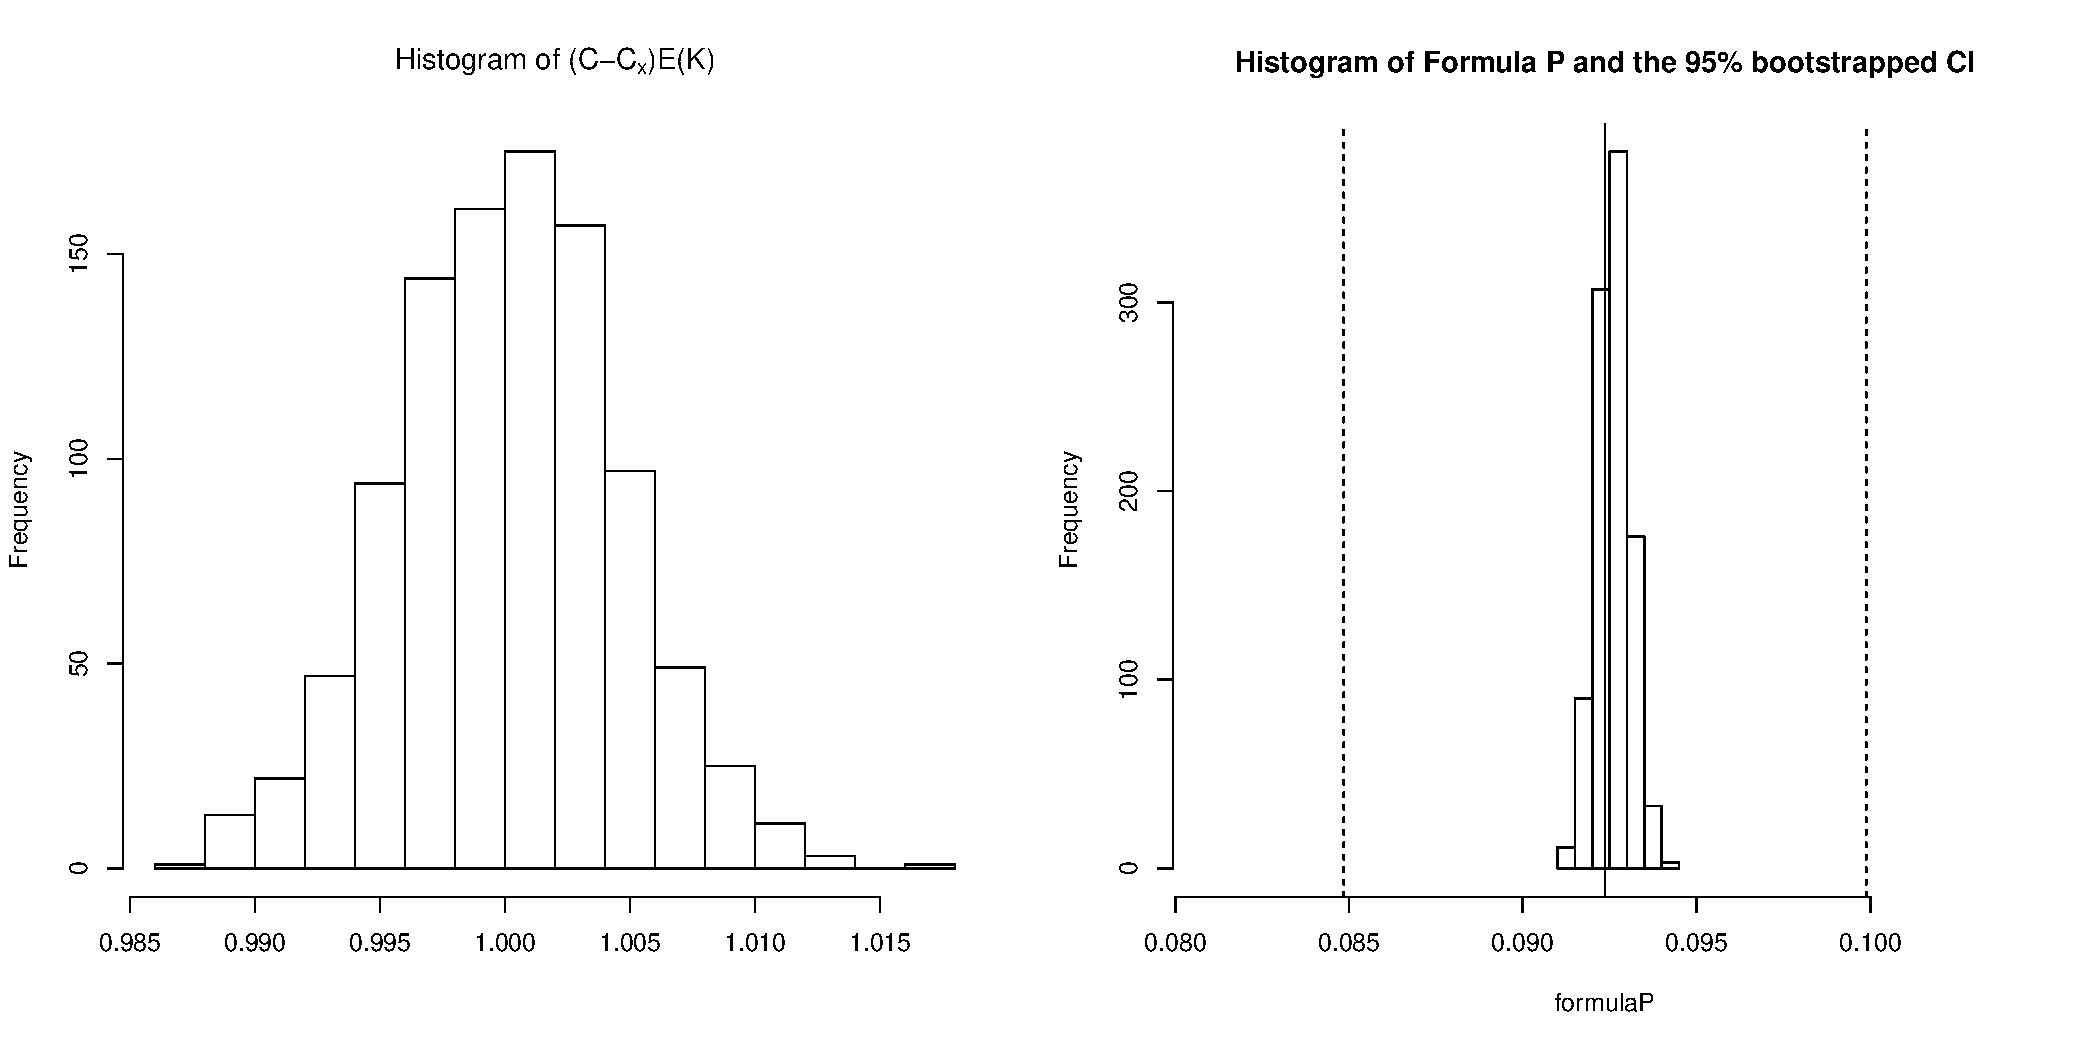
\includegraphics[width=\textwidth]{kpois6}
  \caption{Left: Histogram of $(\wht{C}-\wht{C_x})\wht{\bbe K_i^{(r)}}$. Right: Histogram of the $1000$ estimates from Formula P and the 95\% confidence interval form bootstrap. The two dashed lines are lower and upper bound of the confidence interval and the solid line is the sample variance of $1000$ realization of $\xbar_1-\xbar_2$ multiplied by $n$}
  \label{fig:kpois6}
\end{figure}
We first use $Poisson(6)$ to generate $K_i$, and then $K_i^{(r)},r=1,2$ from the binomial distribution. The left plot in Figure \ref{fig:kpois6} shows that $C-C_x$ is indeed close to $1/\bbe K_i^{(r)}$. The ratio of the two is normally distributed and concentrated around 1. The right plot shows all the $1000$ estimates from Formula P are within the bootstrpped confidence interval. 

%A similar simulation was done for Poisson(6) distribution. Figure~\ref{fig:kpois6} shows the performance of \ref{p_est}. 
%\begin{figure}[!htp]
%  \centering
%  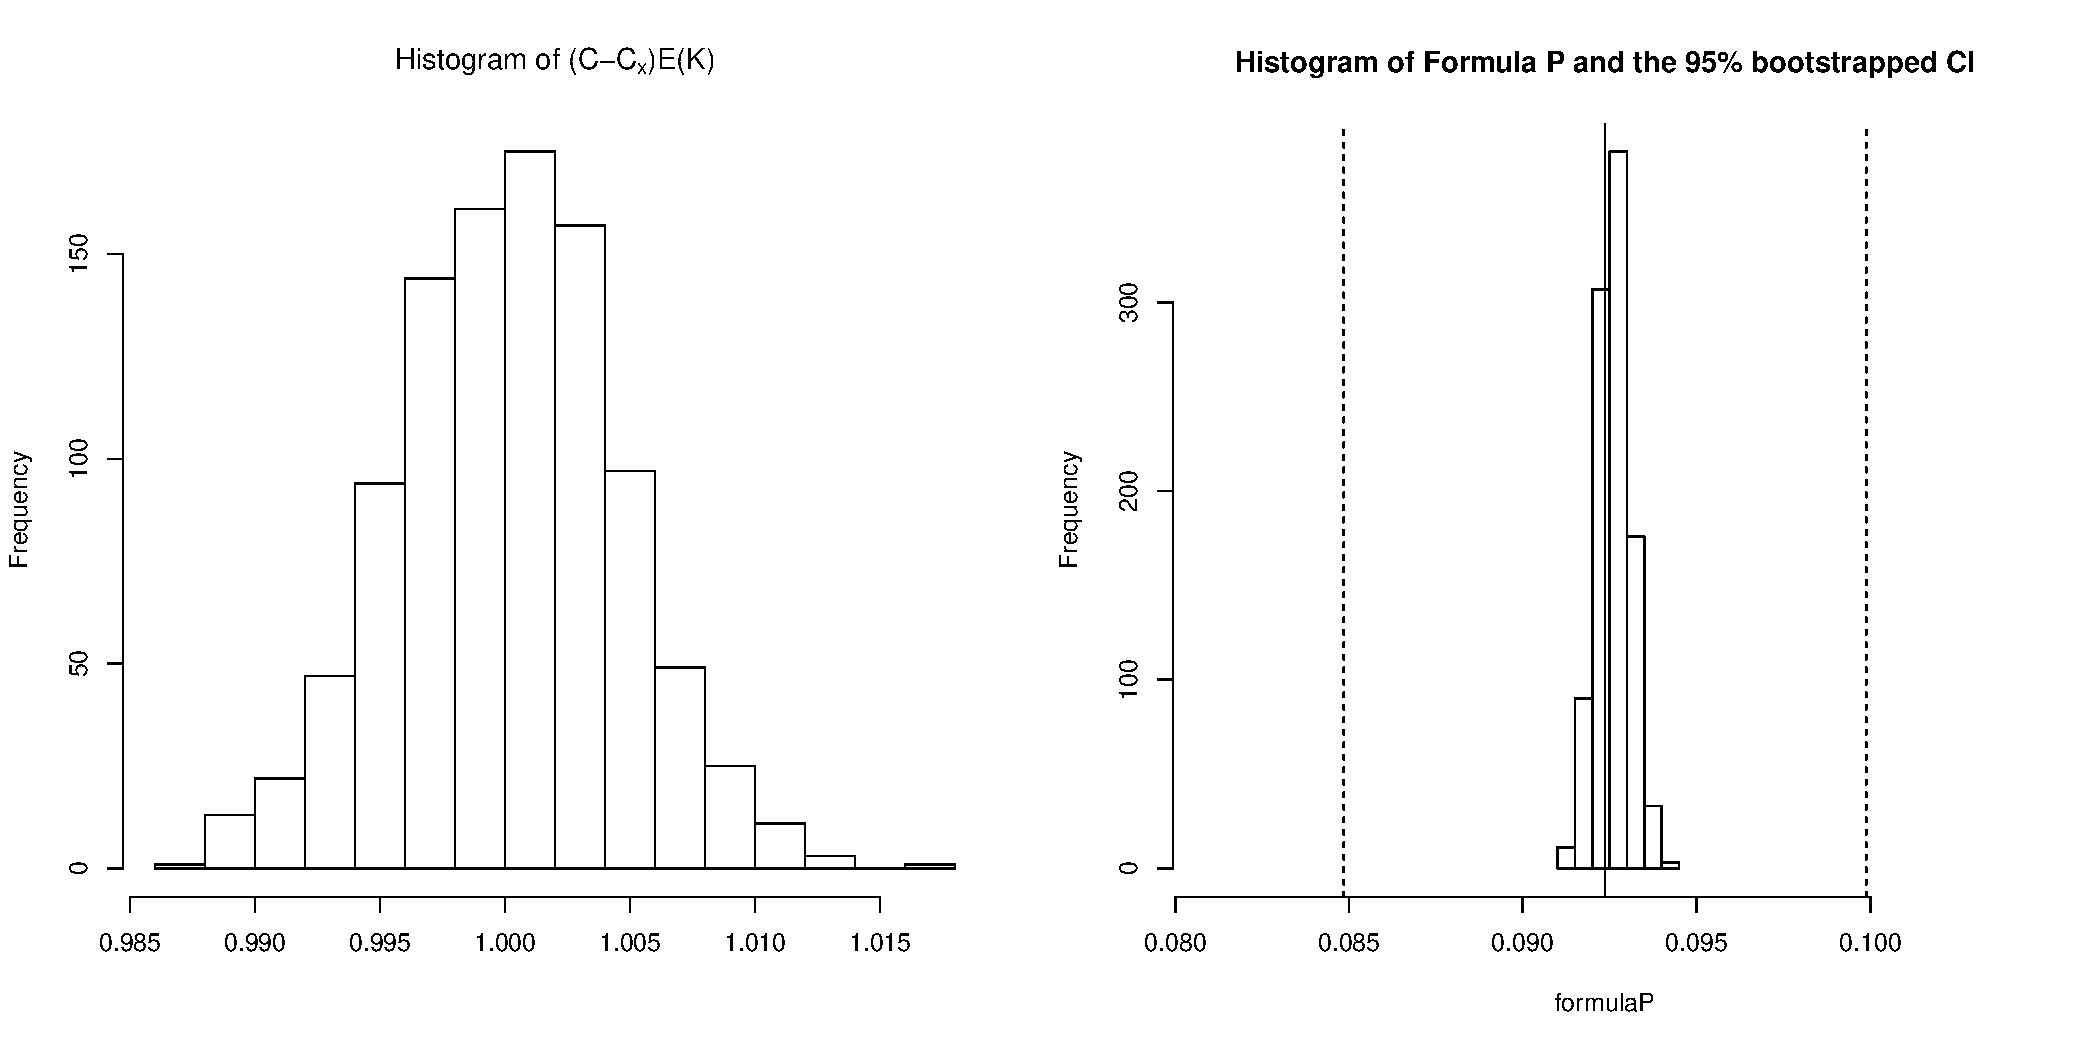
\includegraphics[width=0.5\textwidth]{kpois6}
%  \caption{Histogram of the $1000$ estimates from Formula P and the 95\% confidence interval form bootstrap. The two dashed lines are lower and upper bound of the confidence interval and the solid line is the sample variance of $1000$ realization of $\xbar_1-\xbar_2$ multiplied by $n$}. 
%  \label{fig:kpois6}
%\end{figure}
%\clearpage
\subsubsection{$K_i$ constant case}
In this simulation study, we fixed $K_1=5$. Figure~\ref{fig:kfixed5} shows the performance in this case.

\begin{figure}[!hbtp]
  \centering
  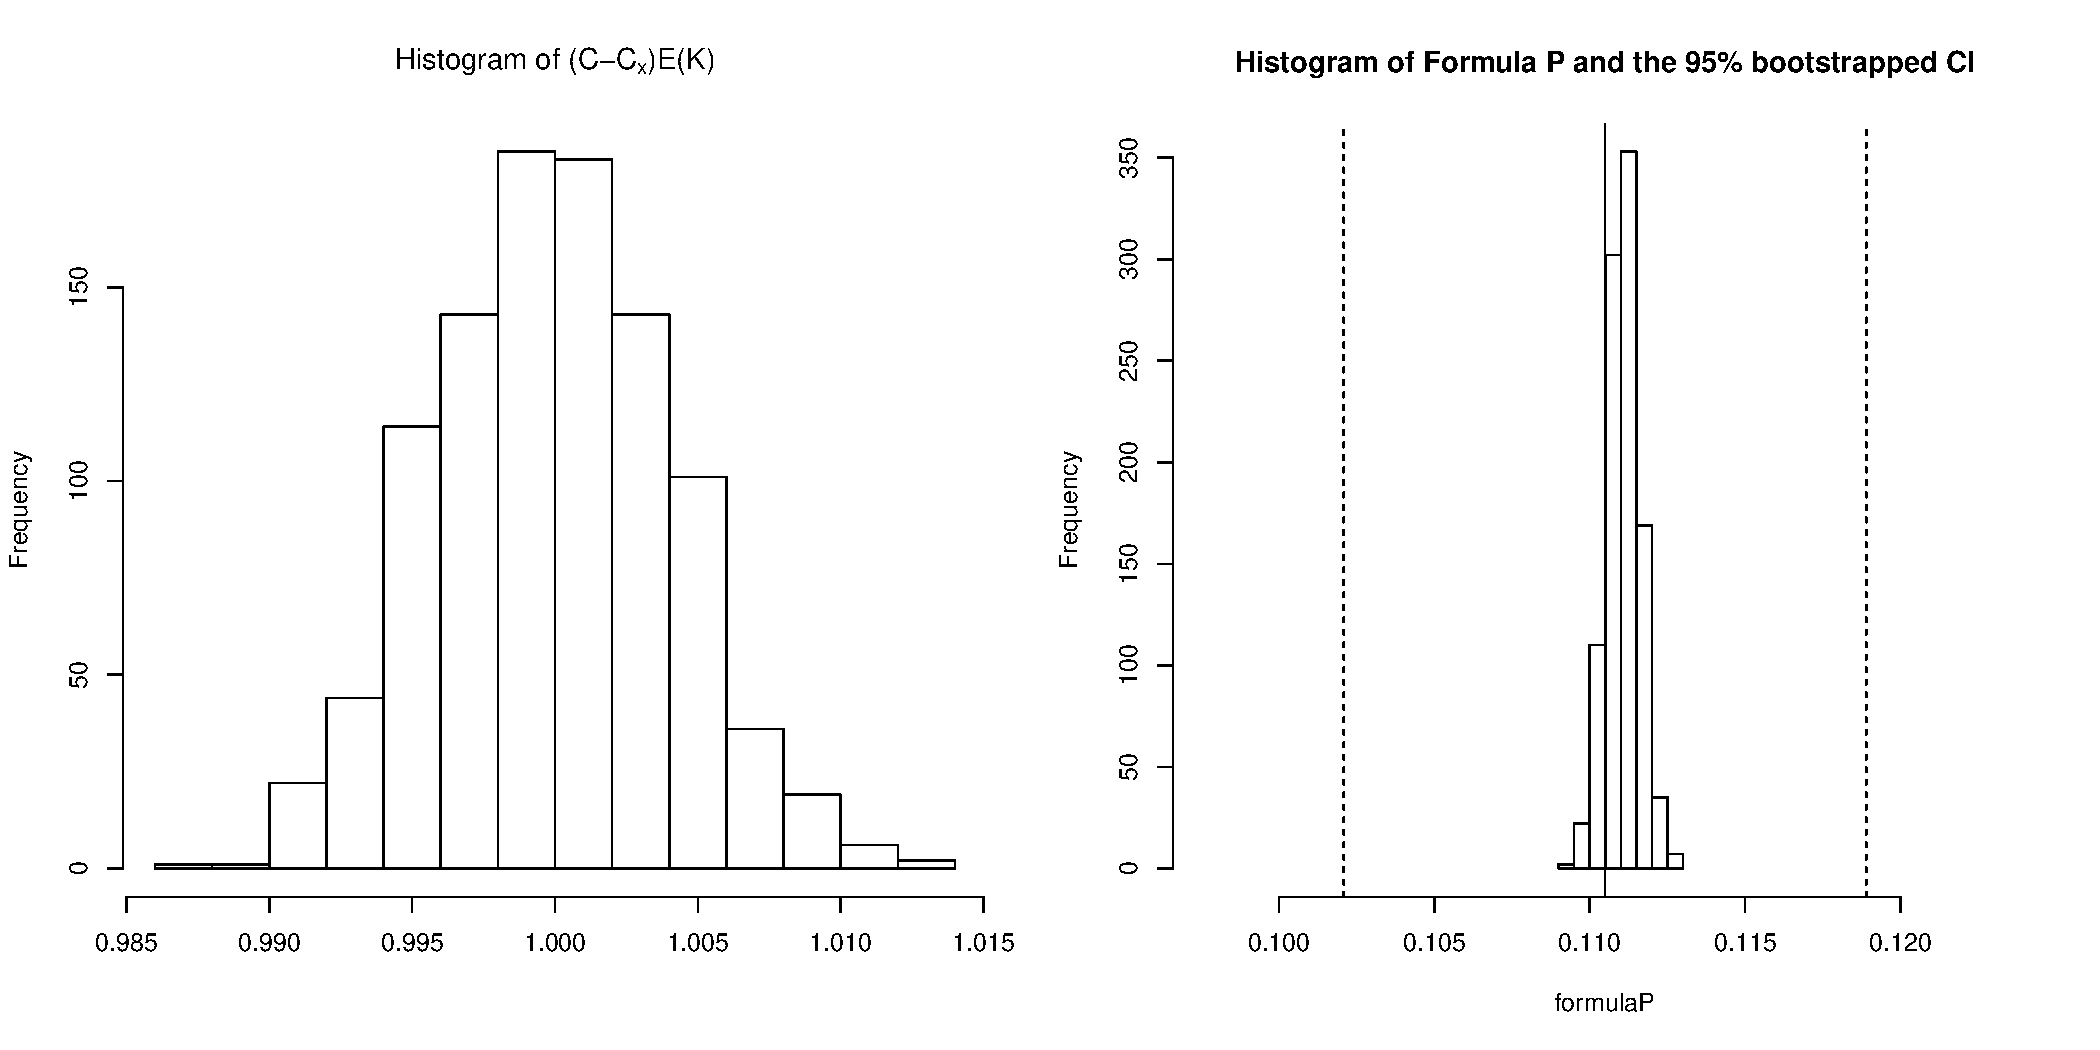
\includegraphics[width=\textwidth]{kfixed5}
    \caption{Left: Histogram of $(\wht{C}-\wht{C_x})\wht{\bbe K_i^{(r)}}$. Right: Histogram of the $1000$ estimates from Formula P and the 95\% confidence interval form bootstrap. The two dashed lines are lower and upper bound of the confidence interval and the solid line is the sample variance of $1000$ realization of $\xbar_1-\xbar_2$ multiplied by $n$}
  \label{fig:kfixed5}
\end{figure}

\section{Conclusion}\label{conclusion}



\bibliography{biblio}
\bibliographystyle{jmr}
\end{document}
